\chapter{Mathematical Model}\label{math_model}
This chapter describes the mathematical model formulated to solve the SEBSRP, presented in \Cref{scope and problem description}. The problem is modeled as a Team Orienteering Problem with additional constraints. The chapter starts with \Cref{assumptions} describing the assumptions made in the mathematical formulation. Further, \Cref{notation} introduces the notation used. \Cref{model} continues by describing the objective function of the model, as well as the constraints the model is subject to. Finally, \Cref{alt_model} presents an alternative model for solving the SEBSRP. 

\section{Assumptions}\label{assumptions}
The reward for rebalancing an e-scooter is decided based on a partition of zones, each with a given demand. Based on this demand, an ideal state is calculated for each demand zone, described in further detail in \Cref{key_input_data}. The demand is considered deterministic and discrete for every instance solved by the model. 

The difference between the ideal state and the current state in a zone, both positive and negative, is called the deviation. It is assumed that no additional e-scooters than the deviation of the zone can be moved to that zone. Hence, if a zone has five e-scooters as its ideal state and currently contains three, only two are allowed to be rebalanced to that zone. Consequently, zones containing more e-scooters than its ideal state will not have any e-scooters delivered to them. The amount of e-scooters needed to reach the ideal state is introduced as additional locations in a zone. As these locations do not contain an e-scooter, neither a battery swap nor pick-up is possible there. These locations are referred to as delivery locations, as mentioned in \Cref{Problem Description}. The introduction of additional delivery locations is visualized in \Cref{fig:deviation}. In the figure, the blue locations represent e-scooters, while the red locations represent empty locations indicating delivery locations. The number of red locations in a zone adds up to the deviation of that zone. Zones without red locations is either in its ideal state, or has too many e-scooters in it.

\begin{figure}[h]
    \centering
    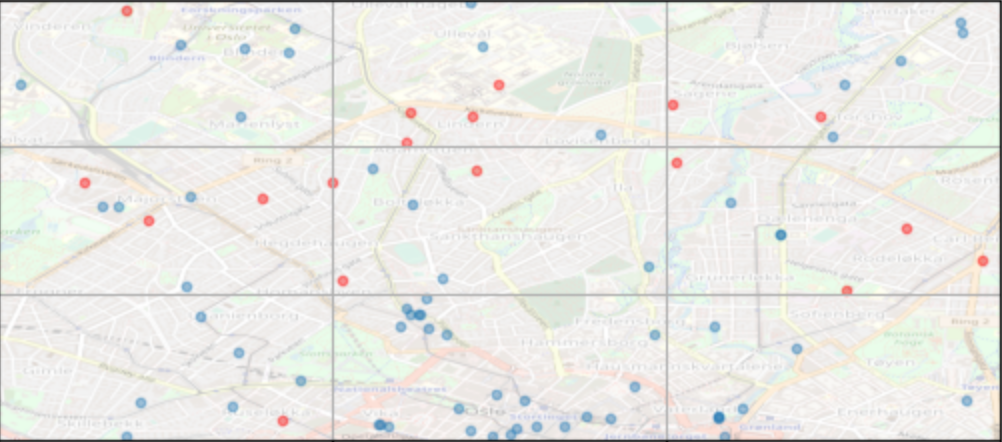
\includegraphics[width=15cm]{Images/deviation.png}
    \caption[The deviation from the ideal state in zones]{The deviation from the ideal state in zones. The red dots, indicating delivery locations, are randomly placed within the delivery zones in this illustration, but could be set manually by operators to fit regulatory and practical limitations.}
    \label{fig:deviation}
\end{figure}

Every location visited gives a reward. The reward contribution of the rebalanced e-scooters are given at the location they are delivered to. Correspondingly, this is where they contribute to increase the availability of e-scooters and satisfy the demand.

\section{Notation}\label{notation}
This section introduces and describes the different sets, parameters, and variables used to formulate the mathematical model in this report. The notation is summarized in its entirety in \Cref{formulation_standard}. 

The formulation consists of a set of locations, with several subsets to define the types of locations. $\mathcal{L}^{+}$ and $\mathcal{L}$, consists of all locations with and without the depot. Sets $\mathcal{L}^{S}$ and $\mathcal{L}^{D}$ denote all e-scooters and delivery locations.

To make the model unable to pick up e-scooters in zones that lack e-scooters, sets to handle zones have to be introduced. $\mathcal{Z}$ contains every zone, while $\mathcal{Z}^{D}$ only consists demand zones, signalling that the zone is below its ideal state. Furthermore, the set $\mathcal{L}_{z}$ is indexed by the zones in $\mathcal{Z}$, and contains every location in a particular zone. 

The last set utilized in the formulation is $\mathcal{V}$, denoting the set of service vehicles. The service vehicles have a battery capacity and e-scooter capacity, denoted $Q^{B}$ and $Q^{S}$ respectively. The battery capacities of the e-scooters in the set $\mathcal{L}^{S}$ are given by the parameters $B_i$.

To constrain the solution from picking up too many e-scooters from the same zone, a parameter, $E_z$, is introduced. $E_z$ denotes the excess of e-scooters in a zone, namely the difference between the number of e-scooters in the zone and its ideal state. 

There is a reward associated with visiting different locations, denoted $R_{i}$. A reward is given if a service vehicle visits a given location, represented by the binary variables $y_{iv}$. As the model rewards every visit to a location, $y_{iv}$ can be seen as a battery swap variable for all locations in the set $\mathcal{L}^{S}$. Additionally, the binary variables $p_{iv}$ are introduced to express the pick-up of an e-scooter. 

The model also utilizes the flow variables $x_{ijv}$. These are binary variables indicating whether service vehicle $v$ travels directly from location $i$ to location $j$. There is a travel time associated with traveling between every location in the set $\mathcal{L}^{+}$. This is denoted $T_{ij}$, and expresses the time service vehicle $v$ uses to move from location $i$ to location $j$. The total duration a service vehicle can operate during a shift is constrained by the length of a shift, denoted $T_{max}$. The relationship between $y_{iv}$ and $x_{ijv}$ is explained in \Cref{fig:y_x_illustration}, where service vehicle number 5 leaves the depot, visits locations 1 and 2, and returns to the depot. 
\\\
\begin{figure}[h]
    \centering
    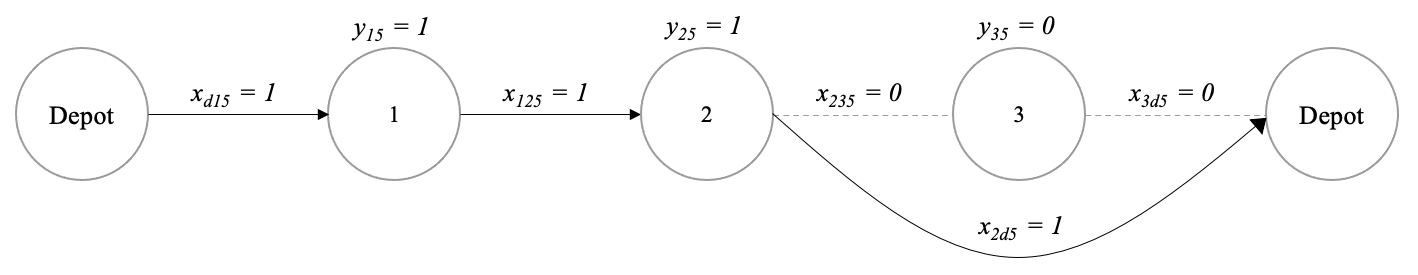
\includegraphics[width=15cm]{Images/y_x_illustration.png}
    \caption[Illustration of an example route for a service vehicle with visits.]{Illustration of an example route for a service vehicle with visits. The $y_{iv}$ can only be $1$ if the location $i$ is visited. Consequently, $y_{35}=0$ as location 3 is not visited.}
    \label{fig:y_x_illustration}
\end{figure}

Every service vehicle has an e-scooter capacity of $Q^{S}$, therefore it is necessary to keep track of the load of each vehicle. $l_{iv}$ denotes the e-scooter load of service vehicle $v$ entering location $i$. \Cref{fig:l_p__illustration} illustrates the relationship between $p_{iv}$ and $l_{iv}$, where service vehicle number 5 performs a pick-up in location 1 and a delivery in location 2. 
\\\
\begin{figure}[h]
    \centering
    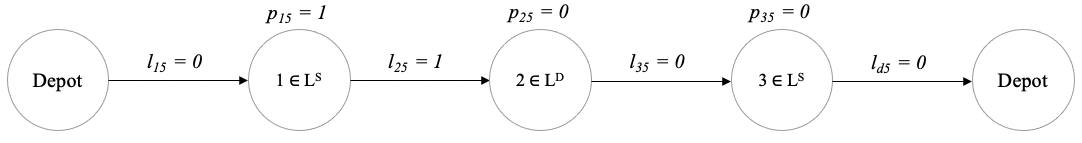
\includegraphics[width=15cm]{Images/l_p_illustration.png}
    \caption[Illustration of an example route for a service vehicle with pick-ups]{Illustration of an example route for a service vehicle with pick-ups. $p_{15}$ is equal to $1$ as an e-scooter is picked up in location 1. The e-scooter is delivered in location 2, which is a delivery location.}
    \label{fig:l_p__illustration}
\end{figure}

Subsequently, the variables $u_{iv}$ are included in the model to avoid subtours in the solution. $u_{iv}$ captures the position of location $i$ in the route of vehicle $v$.

\section{Model}\label{model}

\subsection{Objective function}
\begin{eqnarray}
     \max & \displaystyle\sum_{v\in \mathcal{V}} \displaystyle\sum_{i \in \mathcal{L}} R_{i}y_{iv} - \displaystyle\sum_{v\in \mathcal{V}} \displaystyle\sum_{i \in \mathcal{L}^{S}} B_{i}p_{iv} & \label{eq:objective_5}
\end{eqnarray}

The goal of the objective function is to maximize the reward of swapping batteries and performing rebalancing moves. The model rewards every visit to a location in the set $\mathcal{L}$, as each visit represents a battery swap or delivery of an e-scooter. However, rewarding every visit to a location in the set $\mathcal{L}$, means that, in a rebalancing move, the model rewards both the pick-up and delivery of an e-scooter. The reward should only be given at delivery location, as the reward is intended for the location where the e-scooter is available for use. Hence, the the battery capacity of an e-scooter that is picked up is subtracted from the reward. As a result the model is incentivized to pick up e-scooters with a low battery capacity in a rebalancing move. 

\subsection{Routing constraints}
\begin{eqnarray}
     \displaystyle\sum_{j\in \mathcal{L}^+}x_{djv} = \displaystyle\sum_{i\in \mathcal{L}^+}x_{idv} = 1 & v\in \mathcal{V} \label{eq:const_deopt_5}\\ 
    % A location can only be visited once
	\displaystyle\sum_{v\in \mathcal{V}}y_{iv} \leq 1 & i \in \mathcal{L} \label{eq:const_at_most_once_5}\\
	\displaystyle\sum_{i\in \mathcal{L}^{+}}x_{ikv} = \displaystyle\sum_{j\in \mathcal{L}^{+}}x_{kjv} = y_{kv} & k \in \mathcal{L}^{+}, v\in \mathcal{V} \label{eq:const_connectivity_5}\\
	% Time limit constraint
    \displaystyle\sum_{i \in \mathcal{L}^{+}}\displaystyle\sum_{j \in \mathcal{L}^{+}} T_{ij}x_{ijv} \leq T_{max} & v\in \mathcal{V} \label{eq:const_time_5}
\end{eqnarray}

A set of constraints is introduced  to make sure that every route a service vehicle takes is feasible and resembles the real-world. Constraints \eqref{eq:const_deopt_5} ensure that each service vehicle in the solution starts and ends its route in the depot, denoted $d$. Furthermore, constraints \eqref{eq:const_at_most_once_5} ensure that each location is visited at most once, guaranteeing that each e-scooter only receives one battery swap or rebalancing move. In order to ensure the connectivity of the path for every service vehicle, constraints \eqref{eq:const_connectivity_5} have been introduced. Additionally, to constrain the amount of time a service vehicle can operate during a shift, constraints \eqref{eq:const_time_5} limit the total amount of time to the duration of a shift. 
\begin{eqnarray}
    % No pickup in zones lacking e-scooters
	\displaystyle\sum_{v\in \mathcal{V}}\displaystyle\sum_{i\in \mathcal{L}_z} p_{iv} = 0  & z\in \mathcal{Z}^D \label{eq:pickup_zone_5}\\
	% Cannot pick up more than diff between |Lz| and ideal state
	\displaystyle\sum_{v\in \mathcal{V}}\displaystyle\sum_{i\in \mathcal{L}_z} p_{iv} \leq E_z & z\in \mathcal{Z} \label{eq:pickup_zone_2_5}\\
	% Subtour Elimination
    u_{iv} \leq \displaystyle\sum_{j \in \mathcal{L}^{+}} \displaystyle\sum_{k \in \mathcal{L}^{+}} x_{jkv} &  i\in \mathcal{L}, v\in \mathcal{V} \label{eq:const_subtour1_5}\\
    u_{iv} - u_{jv} +1 \leq (|\mathcal{L}^{+}|-1)(1-x_{ijv})&   i,j \in \mathcal{L}, v\in \mathcal{V}, i \neq j \label{eq:const_subtour2_5}
\end{eqnarray}

Constraints \eqref{eq:pickup_zone_5} ensure that the solution does not pick up e-scooters in zones already below its ideal state. Likewise, constraints \eqref{eq:pickup_zone_2_5} keep the solution from picking up too many e-scooters from the same zone. No more e-scooters can be picked up in a zone than the difference between the number of locations in the zone and its ideal state. Finally, to ensure feasible routes for the service vehicles, constraints \eqref{eq:const_subtour1_5} and \eqref{eq:const_subtour2_5} have been included. These constraints are necessary to prevent subtours in the paths.

\textbf{Capacity constraints}
\begin{eqnarray}
     \displaystyle\sum_{i\in \mathcal{L}^{S}}y_{iv} \leq Q^{B} &   v \in \mathcal{V} \label{eq:battery_const_5}\\
     0 \leq l_{iv} \leq Q^{S} & i \in \mathcal{L}, v \in \mathcal{V} \label{eq:const_vcap_5}
\end{eqnarray}

As the service vehicles only can carry a certain number of batteries and e-scooters, capacity constraints are necessary. Constraints \eqref{eq:battery_const_5} ensures that a service vehicle does not perform more battery swaps than its capacity.  Similarly, constraints \eqref{eq:const_vcap_5}, limits the number of e-scooters in a service vehicles inventory to its maximum capacity. 

\textbf{Inventory constraints}
\begin{eqnarray}
     l_{iv} + p_{iv} - l_{jv} - Q^{S}(1-x_{ijv}) \leq 0 & i \in \mathcal{L}^{S}, j \in \mathcal{L}^{+} \setminus\{i=j\}, v \in \mathcal{V} \label{eq:const_vcap_pickup1_5}\\
     l_{iv} + p_{iv} - l_{jv} + Q^{S}(1-x_{ijv}) \geq 0 & i \in \mathcal{L}^{S}, j \in \mathcal{L}^{+} \setminus\{i=j\}, v \in \mathcal{V} \label{eq:const_vcap_pickup2_5}
\end{eqnarray}

The model also needs to keep track of the inventory of the service vehicles along its route. This is to ensure that every e-scooter that is picked up, also gets delivered at a location. Furthermore, a service vehicle needs to have an e-scooter in its inventory in order to make a delivery. Constraints \eqref{eq:const_vcap_pickup1_5} and \eqref{eq:const_vcap_pickup2_5} forces the variables $p_{iv}$ to become 1 for every location a service vehicle picks up an e-scooter in, while at the same time ensuring that the e-scooter picked up in a location is added to the inventory of the service vehicle.
\begin{eqnarray}
    l_{iv} - y_{iv} - l_{jv} - Q^{S}(1-x_{ijv}) \leq 0 & i \in \mathcal{L}^{D}, j \in \mathcal{L}^{+} \setminus\{i=j\}, v \in \mathcal{V} \label{eq:const_vcap_delivery1_5}\\
	l_{iv} - y_{iv} - l_{jv} + Q^{S}(1-x_{ijv}) \geq 0 & i \in \mathcal{L}^{D}, j \in \mathcal{L}^{+} \setminus\{i=j\}, v \in \mathcal{V} \label{eq:const_vcap_delivery2_5} 
\end{eqnarray}

Additionally, constraints \eqref{eq:const_vcap_delivery1_5} and \eqref{eq:const_vcap_delivery2_5} are needed to determine the inventory of a service vehicle that delivers an e-scooter to a delivery location. 
\begin{eqnarray}
    l_{iv} - Q^{S}(1-x_{div}) \leq 0 & i \in \mathcal{L}, v \in \mathcal{V} \label{eq:const_vcap_depot_out_5}\\
    l_{dv} = 0 & v \in \mathcal{V} \label{eq:const_vcap_depot_in_5}
\end{eqnarray}

As we assume that each service vehicle leaves the depot with nothing but batteries in its inventory, constraints \eqref{eq:const_vcap_depot_out_5} are introduced to force the inventory variables $l_{iv}$ to 0 when entering a location directly from the depot. Finally, in order to make sure that every e-scooter that is picked up, also is delivered, constraints \eqref{eq:const_vcap_depot_in_5} are included.

\textbf{Valid inequalities and symmetry-breaking constraints}
\begin{eqnarray}
     % Symmetry breaking - arcs by vehicle 
	    & \displaystyle\sum_{i\in \mathcal{L}^+}\displaystyle\sum_{j\in \mathcal{L}^+} x_{ijv} \geq \displaystyle\sum_{i\in \mathcal{L}^+}\displaystyle\sum_{j\in \mathcal{L}^+} x_{ij(v+1)} & v \in \mathcal{V} \setminus\{| \mathcal{V}|\} \label{eq:const_number_of_arcs_5}\\
	    % Symmetry breaking - visits by vehicle
	    & \displaystyle\sum_{i\in \mathcal{L}^+} y_{iv} \geq \displaystyle\sum_{i\in \mathcal{L}^+} y_{i(v+1)} & v \in \mathcal{V} \setminus\{| \mathcal{V}|\} \label{eq:const_number_of_visits_5} \\
	    % Symmetry breaking - time used by vehicle 
	    & \displaystyle\sum_{i\in \mathcal{L}^+}\displaystyle\sum_{j\in \mathcal{L}^+} t_{ij}x_{ijv} \geq \displaystyle\sum_{i\in \mathcal{L}^+}\displaystyle\sum_{j\in \mathcal{L}^+} t_{ij}x_{ij(v+1)} & v \in \mathcal{V} \setminus\{| \mathcal{V}|\} \label{eq:const_total_time_used_5}\\
	    %Valid inequalities - back and forth 
	    & \displaystyle\sum_{v\in \mathcal{V}} x_{ijv} + \displaystyle\sum_{v\in \mathcal{V}} x_{jiv} \leq 1 & i,j \in \mathcal{L} \label{eq:const_back_and_forth_5}\\
	    %Valid inequalities - subtour in subset
	    & \displaystyle\sum_{i\in \mathcal{L}} \displaystyle\sum_{j\in \mathcal{L}} \displaystyle\sum_{v\in \mathcal{V}} x_{ijv} \leq |\mathcal{S}|-1  & \mathcal{S} \subseteq \mathcal{L}, |\mathcal{S}|\geq 2 \label{eq:const_subtour_in_set_5}\\
	    %Valid inequalities - arcs less then locations
	    & \displaystyle\sum_{i\in \mathcal{L}} \displaystyle\sum_{j\in \mathcal{L}} \displaystyle\sum_{v\in \mathcal{V}} x_{ijv}  \leq |\mathcal{L}^+|+|\mathcal{V}| \label{eq:const_arcs_less_then_locations_5}
\end{eqnarray}

Constraints \eqref{eq:const_number_of_arcs_5} - \eqref{eq:const_total_time_used_5} are aimed at tightening the solution space of the problem by capturing symmetry in the solutions. They remove the symmetry of vehicles for the number of arcs traversed, the number of visits to locations, and the time used, respectively. Furthermore, constraints \eqref{eq:const_back_and_forth_5} - \eqref{eq:const_arcs_less_then_locations_5} cuts away infeasable parts of the solution space in an attempt to reduce the computational time of the solution. Constraints \eqref{eq:const_back_and_forth_5} cuts away all routes going back and forth between the same two nodes, while constraints \eqref{eq:const_subtour_in_set_5} eliminates subtours in the solution space. Finally, constraints \eqref{eq:const_arcs_less_then_locations_5} constrain the maximum number of arcs to be less than the total number of locations in addition to the final arc back to the depot. An analysis of the reduction of computational time these constraints entails is presented in \Cref{prelim_study}.

\textbf{Non-negativity and binary constraints}
\begin{eqnarray}
    x_{ijv}, y_{iv} \in {0, 1} &   i,j\in \mathcal{L}^{+}, v\in \mathcal{V}\label{eq:const_init_xy} \\
    p_{iv} \in {0, 1} &   i\in \mathcal{L}^{S}, v\in \mathcal{V}\label{eq:const_init_p} \\
    l_{iv} \in \mathbb{N} & i\in \mathcal{L}^{+}, v\in \mathcal{V}\label{eq:const_init_l} \\
    u_{iv} \in \mathbb{N} & i\in \mathcal{L}, v\in \mathcal{V}\label{eq:const_init_u}
\end{eqnarray}

To make sure that only necessary variables are created, the sets used in the model are made as tight as possible. Constraints \eqref{eq:const_init_xy} make the decision of which locations to visit binary over all locations. The locations where a pick-up of an e-scooter is possible are exclusively in the set $\mathcal{L}^{S}$. As a result of this, the variables $p_{iv}$ are made binary over $\mathcal{L}^{S}$. Furthermore, both the inventory variables $l_{iv}$ and the subtour elimination variables $u_{iv}$ are restricted to being integers. Constraints \eqref{eq:const_init_l} and \eqref{eq:const_init_u} initialize them over the sets $\mathcal{L}^{+}$ and $\mathcal{L}$ respectively. 

\section{Alternative Model}\label{alt_model}

In this section, an alternative to the model formulated in the previous subsections is presented. The previous model is henceforth referred to as the standard model. Through the process of modeling the standard model, various areas of improvement have emerged. These include improvements related to reward, time-parameters, subtour elimination, assumptions made, and generally the scope of the problem. The alternative model is formulated based on possible areas of improvement for the standard model, and will in chapter 7 be compared and tested in relation to the standard model. 

\subsection{Purpose of the Alternative Model}

The purpose of the alternative model is to determine if some of the mentioned areas of improvement will improve the performance of the solution. Although not all areas of improvement will be covered in the alternative model, it will handle improvements related directly to the objective function. More specifically it aims to capture the importance of the reward, $R_{i}$, that is given for each location visited. 

In the standard model, the reward is independent of how far away from the ideal state a zone is. This means that whether a location within a specific zone is the only one visited in that zone, or if it is the last of many locations visited, the reward carries the same impact in the objective function. For instance, imagine a zone with an ideal state of 5 with no current e-scooters present and a zone with the same ideal state, but with 4 e-scooters with 100\% battery capacity present. The standard model would give the same reward for moving an additional e-scooter to either of the two zones. In the alternative model, the purpose is that the reward has a more significant impact if the location that is visited is further away from its ideal state. This is, however, only the case for zones not able to satisfy the demand, namely zones lacking e-scooters. 

\Cref{fig:alternative_model} visualizes the deviation from the ideal state. In the figure, the red locations are the possible locations for the delivery of a rebalanced e-scooter. The number of red locations represents the deviation from the ideal state of the specific zone. All blue locations contain an e-scooter with a battery capacity of 100\%, except the two locations marked with 50\% capacity. An e-scooter with 50\% capacity accounts for 0.5 e-scooters in the calculation of the ideal state. The ideal state of all 4 zones is 5. Thus, zone 1 deviates from its ideal state by 3,5 e-scooters, while zone 2 has a deviation of 1,5. In this example, the alternative model would be incentivised to either move an e-scooter from zone 3 or 4 to zone 1, or to swap the battery of the e-scooter with 50\% capacity in zone 1. This is a result of the reward function in the alternative model giving a higher reward for locations in zone 1, as it is further away from its ideal state than the other zones. 
\\

\begin{figure}[h]
    \centering
    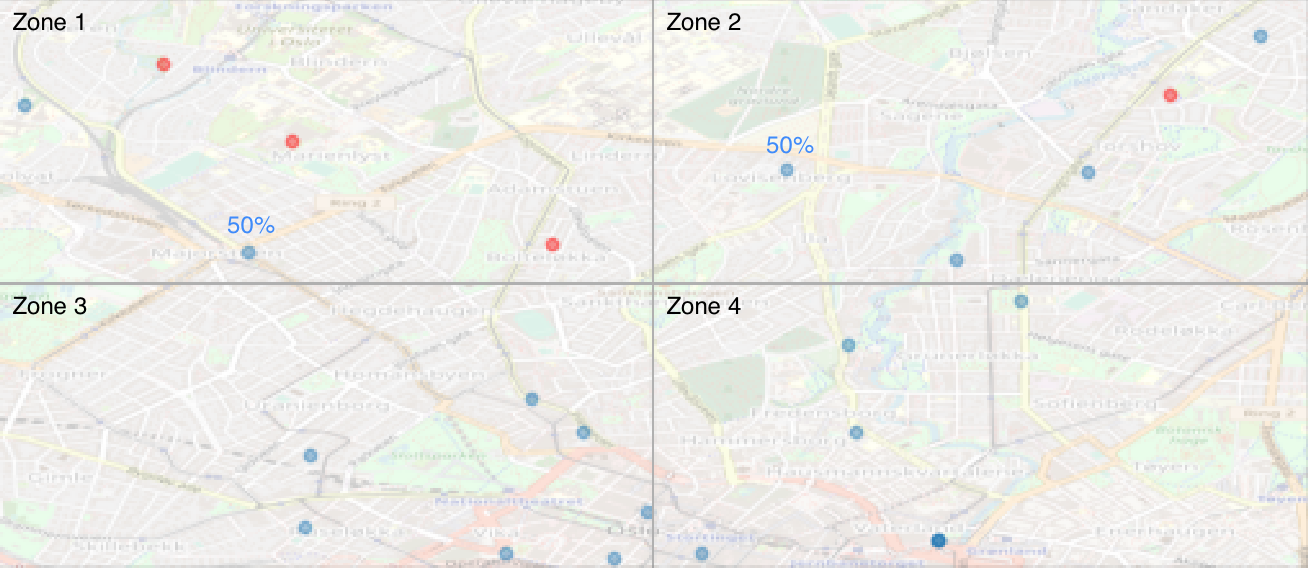
\includegraphics[width=15cm]{Images/alternative_model_ex.png}
    \caption{Example of reward dependent on the deviation from the ideal state}
    \label{fig:alternative_model}
\end{figure}

\break

\subsection{Additional Notation}

The parameter containing the reward, R, is altered from the standard model. In the alternative model, it is denoted $R_{kz}$, and represents the reward for visiting $k$ locations in zone $z$. $w_{kz}$ is a new binary variable that denotes whether or not exactly $k$ locations are visited in zone $z$, and is used in relation to $R_{kz}$ to reward visits to locations. These sets, parameters, and variables are introduced to make the use of a reward function possible and are summarized below. 

\begin{tabular}{p{1.5cm} p{12.5cm}}
    \textbf{Parameters}  \\
    $R_{kz}$ & Reward for visiting $k$ locations in zone $z$\\
    \textbf{Variables}  \\
    $w_{kz}$ & 1 if $k$ locations are visited in zone $z$; 0 otherwise
\end{tabular}

\subsection{Additional Modeling} \label{alt_model_additional_modeling}
\begin{eqnarray}
    \max & \displaystyle\sum_{z\in \mathcal{Z}}\displaystyle\sum_{k=0}^{|\mathcal{L}_z|} R_{kz}w_{kz} - \displaystyle\sum_{v\in \mathcal{V}} \displaystyle\sum_{i \in \mathcal{L}^{S}} B_{i}y_{iv} \label{eq:obj_alt}
\end{eqnarray}

The objective function in the alternative model differs from the standard model, and is shown in Equation \eqref{eq:obj_alt}. The first part of the objective function gives reward depending on the contribution a visit has on the ideal state. In order to further incentivise pick-ups and battery swaps of e-scooters with low battery percentage the model also subtracts the battery percentage of every location visited with an e-scooter, both locations for pick-ups and battery swaps. Thus, the model will prefer to receive a reward for performing an action on e-scooters with a low capacity. 
\begin{eqnarray}
    % Reward based on number of e-scooters handled in zone z
    \displaystyle\sum_{k=0}^{|\mathcal{L}_z|}kw_{kz} = \displaystyle\sum_{v\in \mathcal{V}} \displaystyle\sum_{i \in \mathcal{L}_{z}} y_{iv} -  \displaystyle\sum_{v\in \mathcal{V}} \displaystyle\sum_{i \in \mathcal{L}_{z} \cap \mathcal{L}^{S}} p_{iv} & z \in \mathcal{Z}\label{eq:determine_w} \\
    % Only 1 w in each zone
    \displaystyle\sum_{k=0}^{|\mathcal{L}_z|}w_{kz} \leq 1 & z \in \mathcal{Z}\label{eq:one_w}
\end{eqnarray}

As previously mentioned, the variable $w_{kz}$ keeps track of the number of locations visited in each zone. However, to force it to take this value, a set of constraints has to be introduced. Constraints \eqref{eq:determine_w} forces the value of $w_{kz}$ to the total number of locations visited in zone $z$, except for the locations where an e-scooter is picked up. This is in order for the model to reward only the locations where an e-scooter is delivered in a rebalancing move. The pick-up variables, $p_{iv}$, are only defined over the set $\mathcal{L}^{S}$, leading to the formulation in \eqref{eq:determine_w}. In combination with constraints \eqref{eq:determine_w}, constraints \eqref{eq:one_w} make sure $w_{kz}$ take the correct value for the number of locations visited in a zone.





